
%----------------------------------------------------------------------------------------
%	CHAP Composable R
%----------------------------------------------------------------------------------------

\chapterimage{blue-chapter-head_4-reduced.pdf} % Chapter heading image

\chapter{Composable R}\label{chap:ComposableR}\index{Composable R}\index{R Language}
\section{Overview}
MetaR release 1.5 was the first release to offer a composable R language for MPS (this language is called \textit{org.campagnelab.metaR.R} in MPS, but also simply referred to as ``composable R'', or \textit{compR}). This Chapter explains how to take advantage of this language, what the advantages of a composable R language are, but also describes the current limitations of its implementation.

\subsection{Advantages}
\paragraph{Composable R supports the full R grammar}

The composable R language implemented in MetaR 2.0+ supports  the equivalent of the R language grammar. 
\begin{remark}
We have developed composable R starting with the ANTRL4 R grammar obtained from \url{https://github.com/antlr/grammars-v4/tree/master/r}. This grammar was tweaked to improve priority rules of the parsing rules.
\end{remark}
Because this language is composable, you can design micro-languages to compose with R. An example of micro-language composition, to use the biomart statement described in Chapter~\ref{chap:Biomart}, is shown in Figure~\ref{fig:ExampleRunningComposableRLanguageInMPS}.

\begin{figure}[h!tbp]
  \centering
  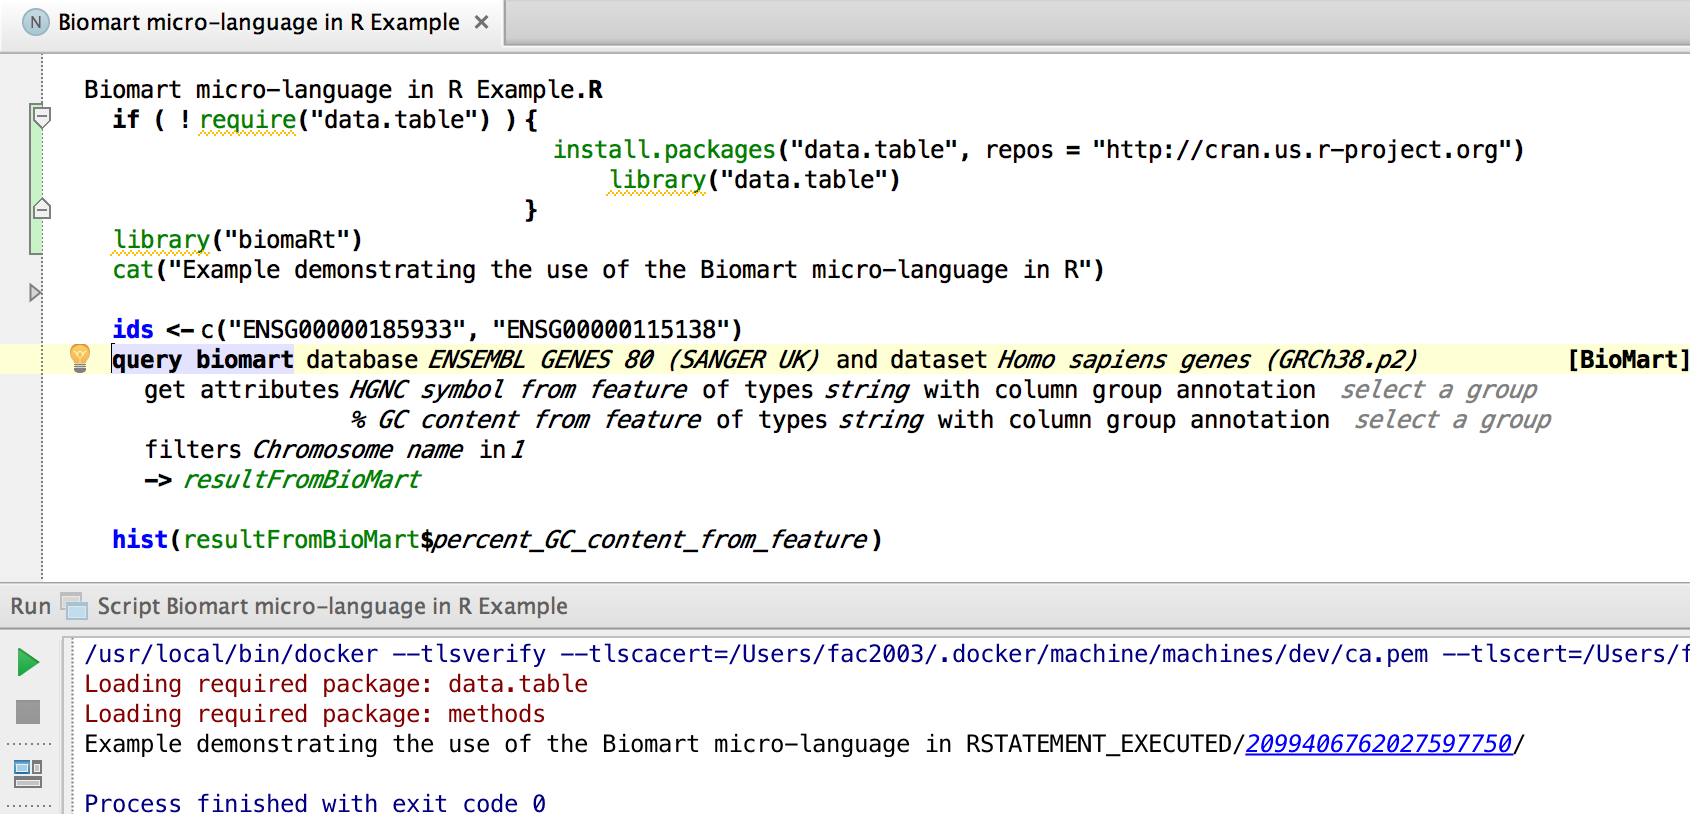
\includegraphics[width=\figWidthWide]{figures/ExampleRunningComposableRLanguageInMPS.png}
\caption[Example of Micro-Language Composition with Composable R.]{\textbf{Example of Micro-Language Composition with Composable R.} In this example, we have composed the MetaR query biomart statement (see Chapter~\ref{chap:Biomart} with the R language).}
\label{fig:ExampleRunningComposableRLanguageInMPS}
\end{figure}


\paragraph{Fluent editing}\index{Fluent editing}

Composable R supports Fluent Editing\footnote{To learn how to implement this feature for your own languages, see~\cite{campagne2015mps}}. We have designed this technique to make it easier to paste an R code fragment from text into an R script. The technique is also very useful to enter complicated R expressions more quickly than possible with the MPS  projectional editor. Read on to learn how to use it.

Fluent editing can be used in any context where an expression or function parameter declaration is expected into a composable R script.  For instance, assume that you have created a new R script. Place the cursor on a new line of this script, and  paste: 
\begin{lstlisting}
c(1,2,3,4,5)
\end{lstlisting}
Immediately after you pasted this expression, fluent editing will parse the expression and translate it to composable R. Since \texttt{c} is an identifier that refers to a function, you will see the color of the \texttt{c} letter change from blue (an identifier not linked to a declaration) to the color green  (used to indicate identifiers linked to a declaration). In this case, the function identifiers becomes linked to the function declaration, in one of the package stubs shipped with MetaR. 

You can paste several lines of R code that will be parsed and inserted into the program in a similar manner. Note that you do not need to paste any text and may just start typing into any location that accepts an R expression (\texttt{Expr} concept in the \textit{org\allowbreak{}.campagnelab\allowbreak{}.metaR\allowbreak{}.R} language). Press return when you are satisfied the text you typed is parseable and the code will be inserted into the script. Use the auto-completion menu to select Fluent code entry if the text you type generates any ambiguity and press return to parse the text and insert the parsed program into the script. 

\begin{remark}
Pasting expressions and parameter declarations should be sufficient to paste in most contexts given the simple grammar of the R language. Let us know if you find that pasting does not work in some context where you would expect it to. In such cases, try pasting a larger piece of R code that contains the one you need to paste. Pasting should work if this larger piece is an R expression. 
\end{remark}


\subsection{Limitations}

\paragraph{Composable R is not an R IDE}

The goal of this language is not to replace an R integrated development environment (IDE) (e.g., RStudio). A number of capable IDEs for the R language already exist, and it is not our intention to develop another one.  Composable R is developed as a research tool that helps us explore the advantages and limitations of language composition for data analysis.

This being said, composable R  provides some features commonly found in good IDEs, including:
\begin{itemize}
  \item auto-completion for function and identifier names.
  \item auto-completion for language keywords and constructs.
  \item navigation to function definition or previously defined identifier, within a script.
  \item ability to define intentions to automate modifications of R code and scripts.
  \item automatic refactorings (renaming an identifier automatically renames all references to this identifier).
  \item You can run R scripts directly from within MPS. When you run, composable R scripts are generated to pure R scripts and the scripts is executed either with a local installation of R or with a Docker container. 
\end{itemize}



\noindent{}However, the following features typically found in IDEs are not supported in MetaR:

\begin{itemize}
  \item An interactive R console,
  \item An R debugger,
  \item A view of plots or tables created by a script. 
\end{itemize}

For these reasons, we recommend using Composable R together with a good R IDE.

\begin{remark}
We have started to address the third limitation in MetaR 2.0. For instance, we offer the ability to preview plots directly inside an R script by using the MetaR \texttt{multiplot} statement. 
\end{remark}

\section{RScript Root Node}
To create a composable R script in a model, make sure \textit{org.campagnelab.metaR.R} is declared in the list of Used Languages. Then select the model, right-click and do \menu{o.c.metaR.R.RScript}. This will create a root node, such as shown in Figure~\ref{fig:NewRScriptRootNode} where you can type expressions in the R language. 

\begin{figure}[tbhp]
  \centering
  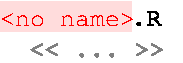
\includegraphics[width=\figWidthTiny]{figures/NewRScriptRootNode.pdf}
\caption[New RScript Root Node]{\textbf{New RScript Root Node.} Press \keys{\return} over the \mpsplaceholder{} to enter new expressions in the script. Enter at least a single new line before pasting code.}
\label{fig:NewRScriptRootNode}
\end{figure}

\begin{remark}
Since version 2.0, you can compose MetaR statements into a composable R script. To do this, import the language \textit{org.campagnelab.metar.R.metar} and use the \texttt{metar} auto-completion. This will create a wrapper for a MetaR statement that lets you insert any MetaR statement into the script. 
\end{remark}

\subsection{Example}
Figure~\ref{fig:UnitedNationPlotScript} shows an example of an RScript written with MetaR. Note the \texttt{Save Session} and \texttt{installOrLoad} statements at the top to support instant refresh. Similarly, the \texttt{export plot} statement wraps the code that produces the plot into a named block of code and makes it possible to refer to the plot in the \texttt{multiplot} statement (composed from MetaR)

\begin{figure}[h!tbp]
  \centering
  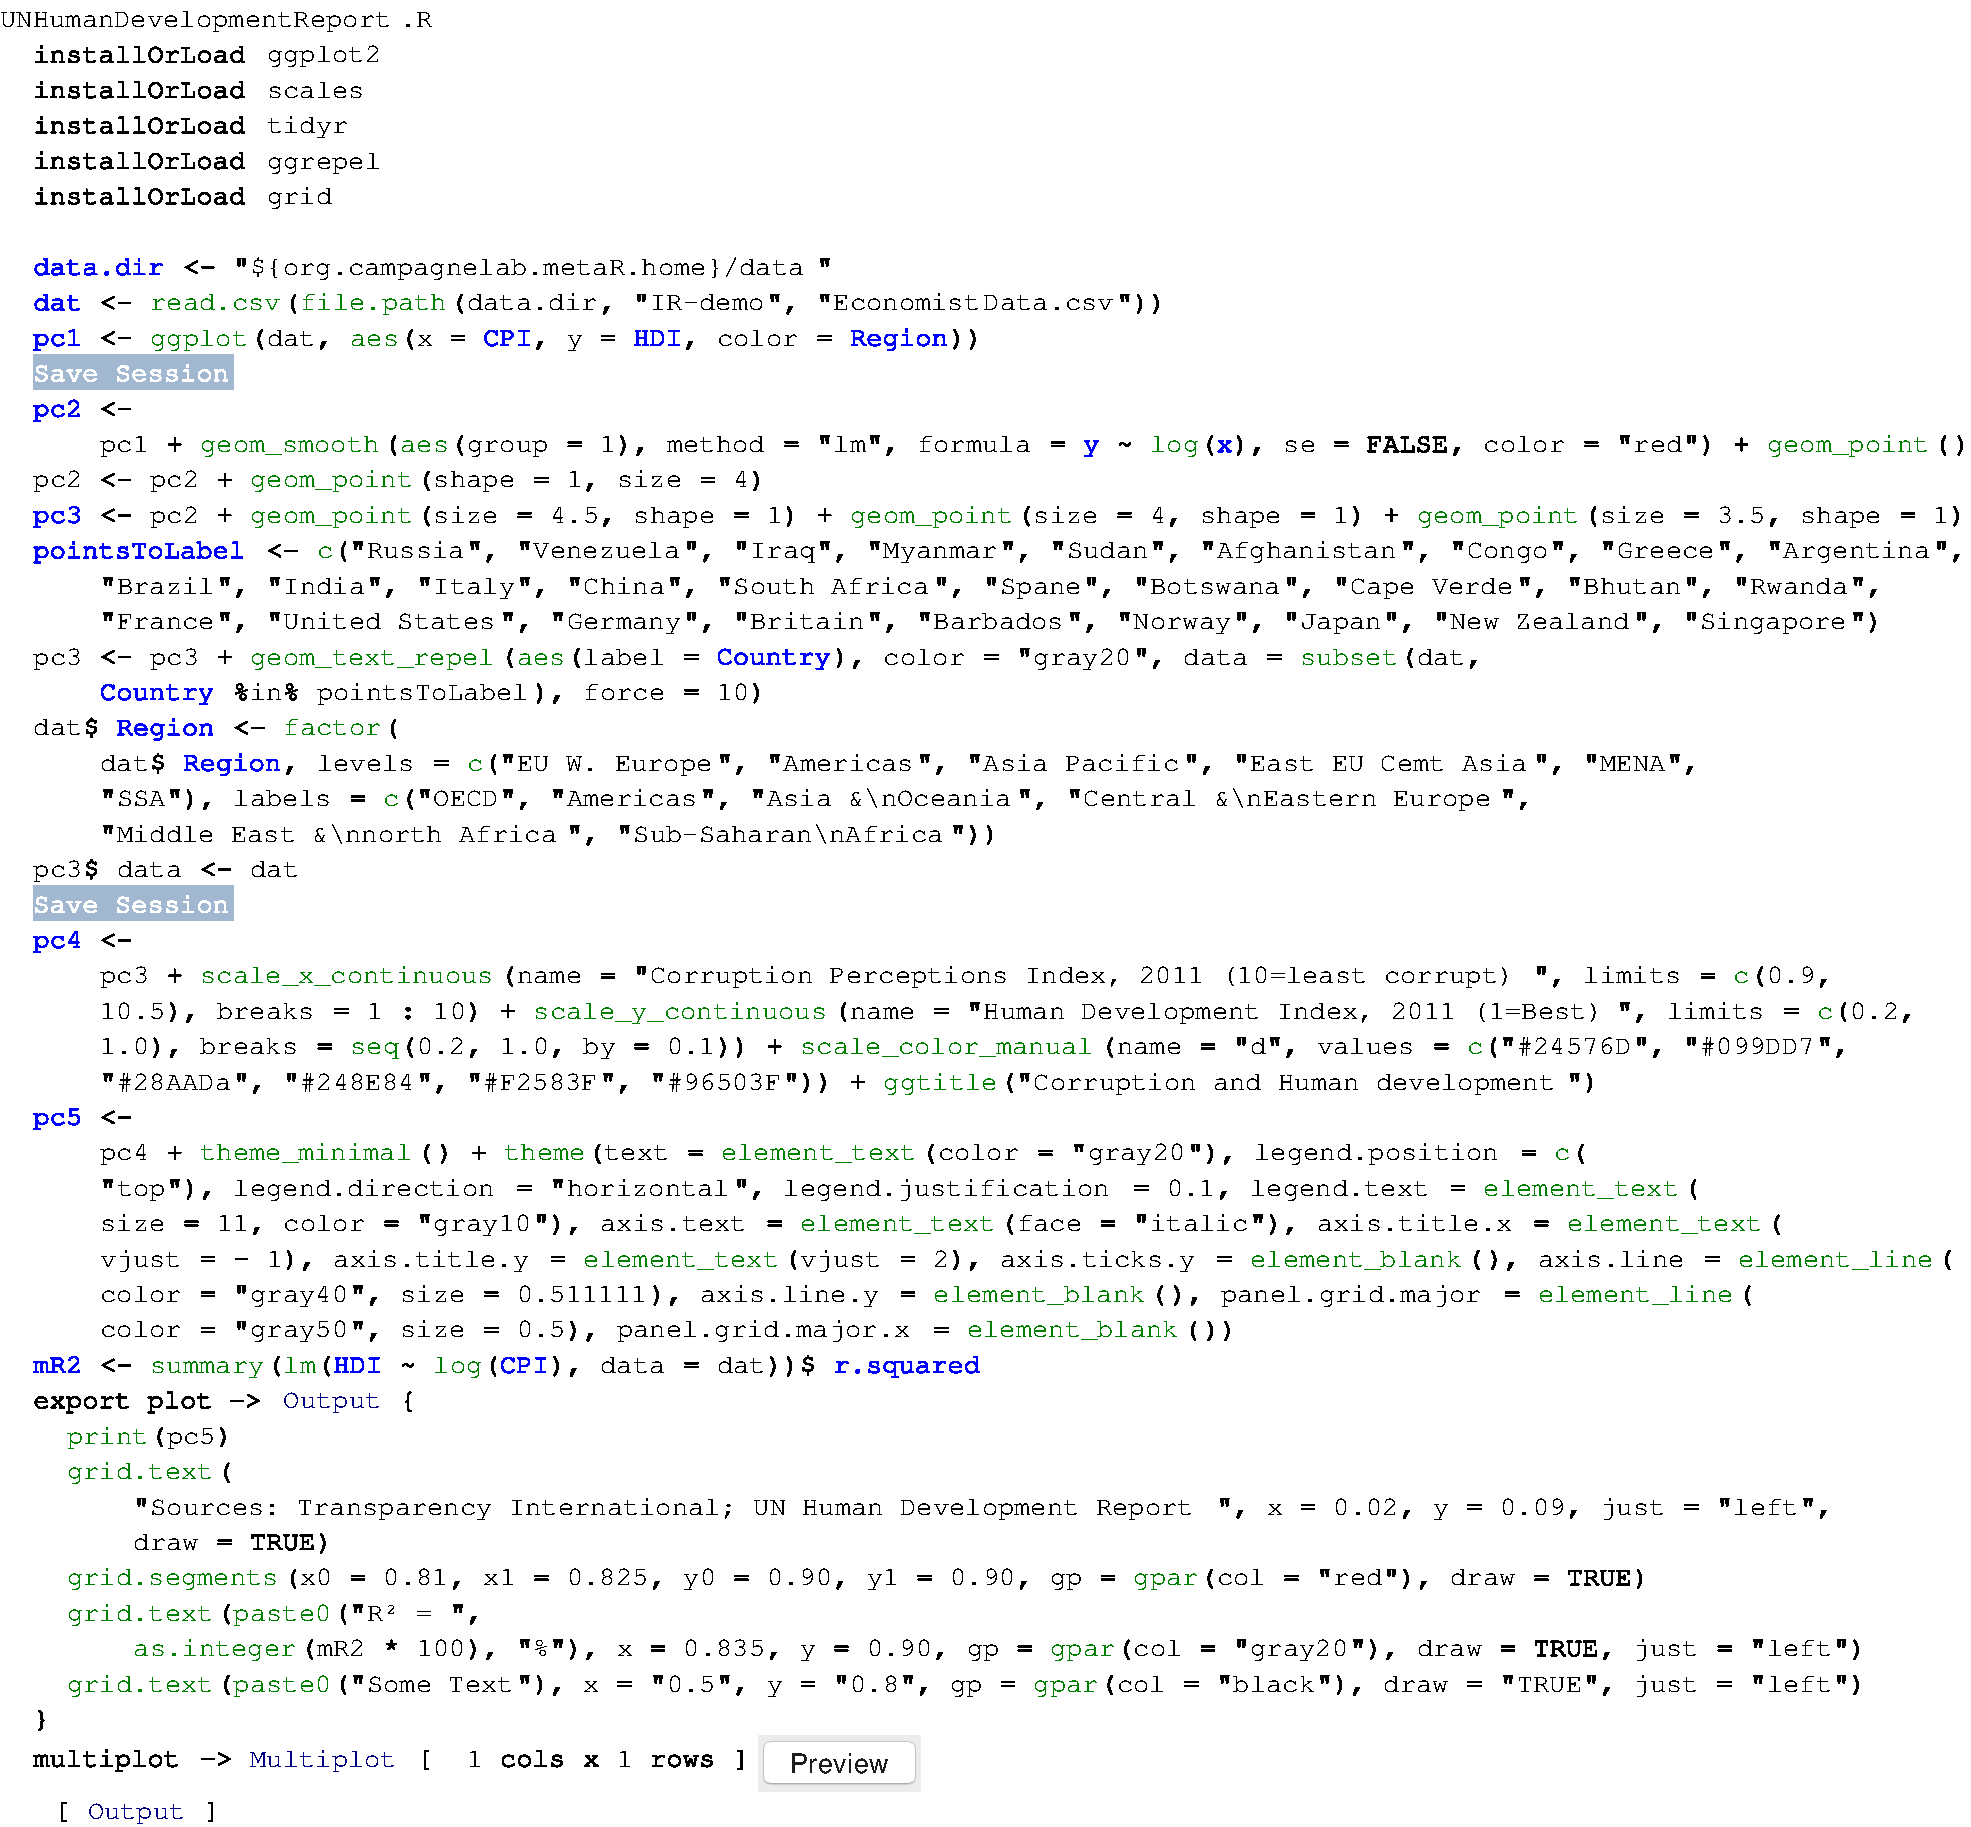
\includegraphics[width=\figWidthWide]{figures/UNPlot.pdf}
\caption[United Nation Development Plot script with MetaR.]{\textbf{United Nation Development Plot script with MetaR.} This script was pasted into MetaR from the code example available at \url{http://tutorials.iq.harvard.edu/R/Rgraphics/Rgraphics.html}. Note the use of language composition that adds new statements and associated semantic to regular R code.}
\label{fig:UnitedNationPlotScript}
\end{figure}

\subsection{Execution}
RScript root nodes can be executed directly from within MPS. Select an RScript, right-click and do Run 'Script <name>', where name is the name of the RScript you wish to execute. Notice that you can provide program parameters in the Run Configuration dialog. Docker execution (see Chapter~\ref{chap:DockerIntegration} is also supported).

Since MetaR 2.0\index{New in MetaR 2.0}, composable R scripts support instant refresh. Changing the script will trigger re-runs of the script in the background and will update plots and tables in real time. See Chapter~\ref{chap:InstantRefresh} for details. 

\section{installOrLoad statement}\index{installOrLoad}\label{sec:installOrLoad}
This statements conveniently loads a package, or installs and loads it if the package was not present in the R distribution used to execute the script. This statement takes a single argument: the name of the package/library to load. The inspector also offer the ability to customize the CRAN repository/mirror used to download and install  the package. 
The following statement:
\begin{lstlisting}
installOrLoad session
installOrLoad ggplot2
\end{lstlisting}
will generate the following R code:

\begin{lstlisting}
installOrLoad<-function (lib,
		repo="http://cran.us.r-project.org")   {
		if(!require(lib,character.only=TRUE)){
			install.packages(lib,repos=repo)
  			library(lib,character.only=TRUE)
  		}
  }
installOrLoad("session")
installOrLoad("ggplot2")
\end{lstlisting}
and result in installing and or loading the session and ggplot2 packages.

\section{Package Stubs}
The composable R language also defines the Stub root node, discussed in Section~\ref{sec:Stubs}. Stubs contain description of the functions and function paramters offered by R packages and can be created automatically from the name of the package.




